% 1. add ip: redpitaya_converters
% 2. physical interface: CTRL-t to Make External
% 3. adc_rst_i -> periph_reset of rst_ps
% 4. configure redpitaya_converters to 14 or 16 bits
% 5. dataAout -> Ain and same for B
% 6. left window: sources -> constraints -> constrs_1 Right click: add Sources -> Add or
%    Create Files -> fpga_ip -> redpit_converters -> adc or adc16 in addition to redpitaya_converters

\documentclass[10pt,oneside]{article}
\usepackage{makeidx,anysize,mflogo,xspace,float,epsfig,url}
\usepackage{amsmath,amsfonts,amssymb,a4wide} 
\urlstyle{sf}
\usepackage{hyperref}
\usepackage{graphicx}
\usepackage{graphics}
\usepackage{float}
\usepackage{caption}
\usepackage{colordvi} %??
\usepackage{listings} 
\usepackage{subfigure}
\usepackage{subfloat}
\usepackage{xcolor}
%\usepackage[labelsep=quad,indention=10pt]{subfig}
\definecolor{grey}{rgb}{0.95,0.95,0.95} % on définit la couleur grise
	% (c'est un gris très clair)
	\definecolor{red}{rgb}{1.0,0.0,0.0} 
	\definecolor{green}{rgb}{0.0,1.0,0.0}
	\definecolor{blue}{rgb}{0.0,0.0,1.0}
	\lstloadlanguages{bash,Java,C,C++,csh,make,sh}%%[Visual]Basic,xml}
	\lstset{frame=none,basicstyle=\footnotesize,breaklines,tabsize=2,captionpos=b,
		prebreak={\hbox{$\rightarrow$}},postbreak={\hbox{$\hookrightarrow$}},
		showstringspaces=false,backgroundcolor=\color{grey}\bfseries,
		keywordstyle=\color{blue},commentstyle=\color{green}\textit,
		stringstyle=\color{red}\ttfamily,abovecaptionskip=2pt,aboveskip=0pt,
		belowskip=0pt,belowcaptionskip=0pt,numbers=none,columns=fullflexible, backgroundcolor=\color{grey}}
%left,numberstyle=\footnotesize,
%		stepnumber=2,numbersep=1pt}
\graphicspath{{./figures/}}

\begin{document}


\begin{center}
{\bf \Large Redpitaya: first Vivado project example, using the RF ADC and DAC} \\ \ \\
G. Goavec-M\'erou \\ \ \\ \today
\end{center}

This documents aims at providing basics on:
\begin{itemize}
\setlength\itemsep{0em}
\item creating a basic Vivado project and the associated block design,
\item adding IP and connections between these processing blocks as well as towards the FPGA pins,
\item generating the bitstream,
\item converting the bitstream to a format usable with GNU/Linux and configuring the FPGA.
\end{itemize}

This presentation will aim at connecting the Redpitaya radiofrequency ADC 
output to the DAC input (Fig. \ref{bloc_design_final}).

\begin{figure}[h!tb]
\begin{center}

\includegraphics{objective.png}
\end{center}
%\hspace{-1cm}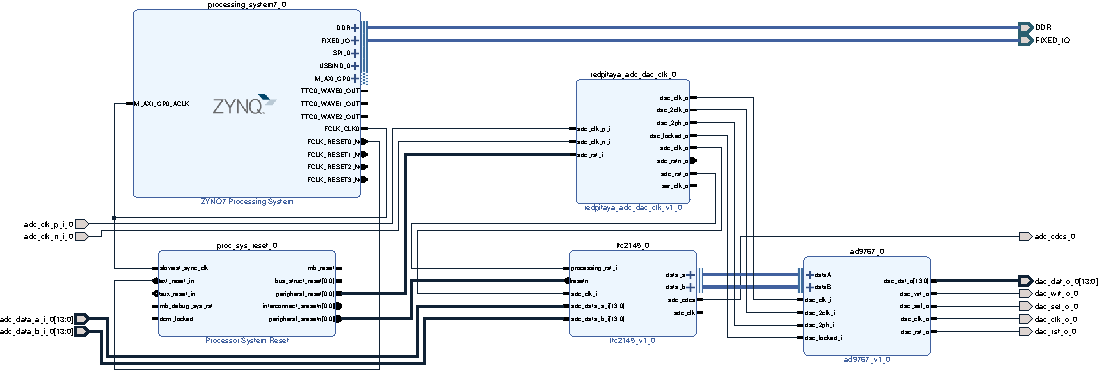
\includegraphics[width=0.97\textwidth]{./block_design.pdf}
\hspace{-1cm}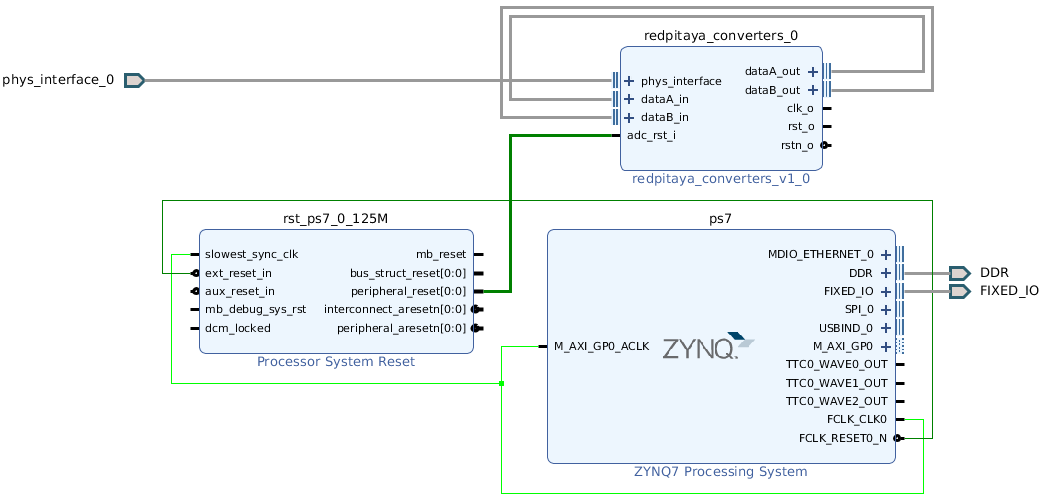
\includegraphics[width=0.97\textwidth]{combinedADC_DAC.png}
\caption{Objective of the tutorial (top) and block design (bottom) including the processor, and
the combined ADC/DAC block including clocking circuit.}
\label{bloc_design_final}
\end{figure}

%\section{File structure}
%
%\begin{lstlisting}
%mkdir my_project
%mkdir -p my_project/app my_project/modules
%\end{lstlisting}

% JMF : je commente, je ne comprends pas ce qu'est cette ligne ci-dessous ni la suite
%vivado settings.me
%\begin{lstlisting}
%VERS=2016.2
%BASE_DIR="/data/Xilinx/Vivado"
%source ${BASE_DIR}/${VERS}/settings64.sh
%export LD_LIBRARY_PATH=${BASE_DIR}/${VERS}/ids_lite/ISE/lib/lin64:$LD_LIBRARY_PATH
%export LANG="en_US.UTF-8"
%\end{lstlisting}

% JMF pour un tuto, je pense qu'on peut se limiter a l'install par default. Le mec qui met dans /data sait se demerder
%\begin{lstlisting}
%source /opt/Xilinx/Vivado/settings64.sh
%vivado
%\end{lstlisting}

\section{Creating the design}

Creating a new design for the Redpitaya requires configuring a project for
the Zynq 7010 embedded on the board (Figs. \ref{createProj1}, \ref{createProj_selectType}, 
\ref{createProj_selectpart} and \ref{createProj_summary}): despite not being 
defined in Xilinx Vivado, we provide manually the proper Zynq declination
instead of the platform settings (Fig. \ref{createProj_selectpart}).

Such a result is achieved by selecting a {\tt RTL Project} so that all additional
configurations are performed manually. The option {\em Do not specify sources at this time} 
prevents {\tt Vivado} from asking the list of source files at the creation of the project
(Fig. \ref{createProj_selectType}).

\begin{figure}[h!tb]
\begin{center}
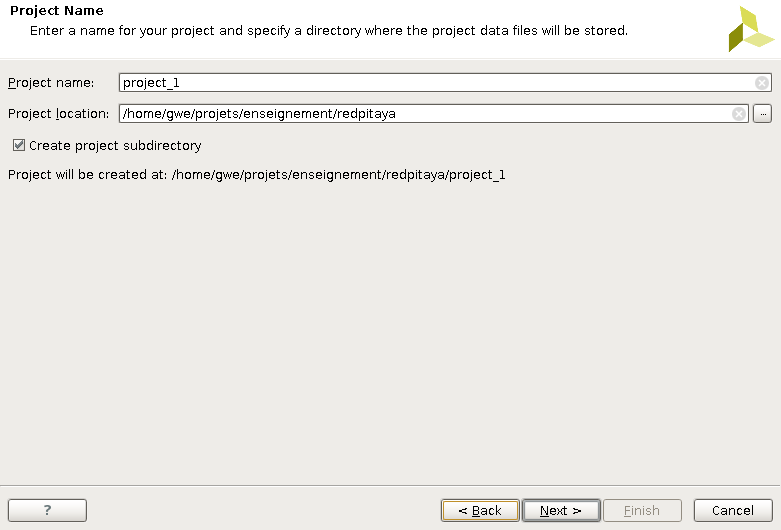
\includegraphics[width=0.5\textwidth]{./createProj1.png}
\end{center}
\caption{Selecting the project name and storage location}
\label{createProj1}
\end{figure}

\begin{figure}[h!tb]
\begin{center}
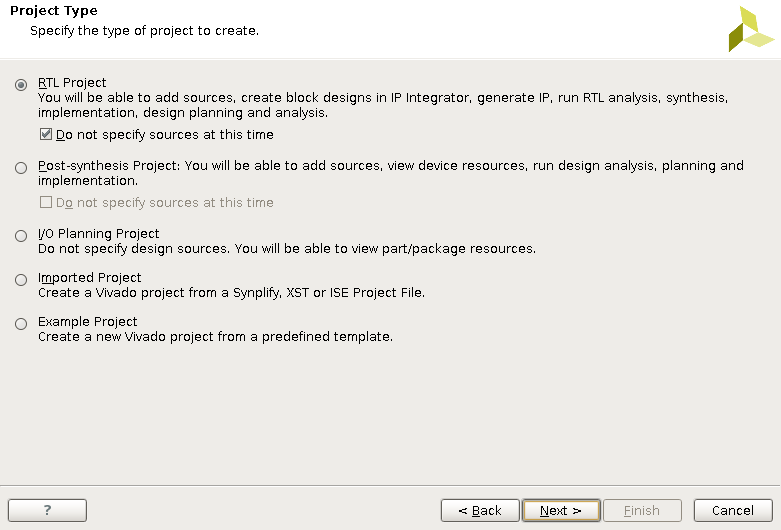
\includegraphics[width=0.5\textwidth]{./createProj_selectType.png}
\end{center}
\caption{Selecting the project type.}
\label{createProj_selectType}
\end{figure}
\begin{figure}[h!tb]
\begin{center}
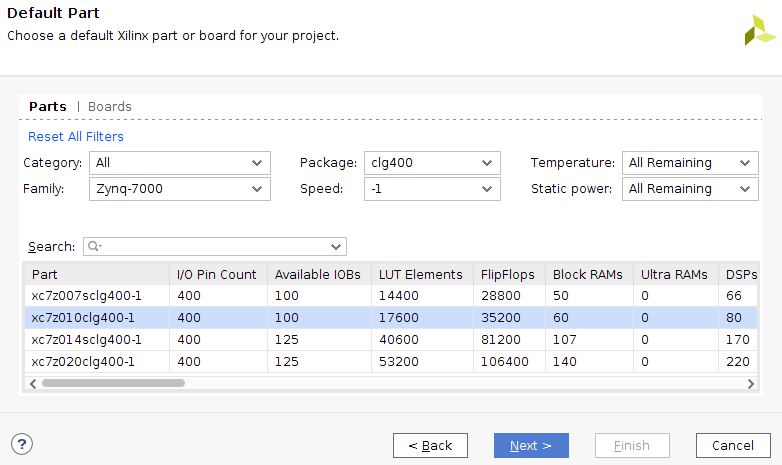
\includegraphics[width=0.7\textwidth]{./createProj_selectPart2019.png}
\end{center}
\caption{Selecting the Zynq SOC type: the Redpitaya is fitted with a {\tt xc7z010clg400-1} model
of the Zynq, hence a Zynq-7000 in a ``clg400'' package, and a speed grade set to -1.}
\label{createProj_selectpart}
\end{figure}
\begin{figure}[h!tb]
\begin{center}
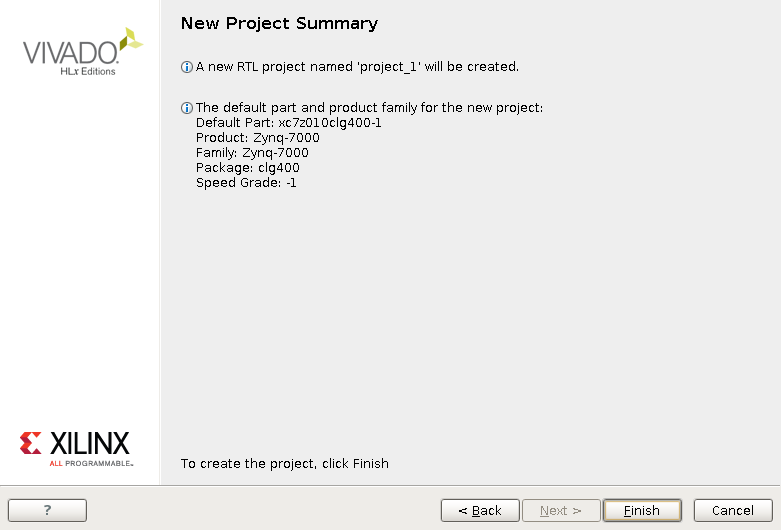
\includegraphics[width=0.5\textwidth]{./createProj_summary.png}
\end{center}
\caption{Fen\^etre r\'ecapitulative.}
\label{createProj_summary}
\end{figure}

\section{Creating the block design}

The classical approach offered by Vivado is to assemble blocks graphically: while we
shall depart later from this approach for large designs, we will use it for the smaller
designs of the first tutorials. Assembling IPs graphically is achieved using the
{\em block design} tool.

In the left menu, double click on {\em Create Block Design}. Selecting the design
name does not really matter but will define the final bitstream name: for consistency
sake we {\bf advise to use the same name than the name of the project}.

The first item to be added is the {\em processing system} (representing CPU in the
block design). Such a result is achieved by displaying ({\tt CTRL + i} shortcut) a
window allowing for the selection of all available IPs. In the list, add {\em ZYNQ7 
Processing System} (search keyword {\tt zynq}). Failing to add this IP, even if not needed,
will result in a system freeze when configuring the FPGA from GNU/Linux.

Once this block has been added, a green horizontal bar appears with the text
{\em Run Block Automation}. Running this option will route the few mandatory connections.

At the beginning of a project creation {\em block design} has no knowledge of the
Redpitaya hardware configuration (amount of RAM, peripherals ...): defining such
a configuration of the processing system is needed for further work. Such a result
is achieved by double-clicking on the {\em processing system} block: on top
of the newly created window, in the {\tt Presets} menu, select {\em Apply configuration} 
and load the configuration file {\tt redpitaya.tcl} (or {\tt redpitaya16.tcl} for the
16-bit Redpitaya version
\footnote{In case of the 16-bit Redpitaya, we wish to echo the 16-bit ADC measurement to
the 14-bit DAC. A bit-shift -- \url{https://github.com/oscimp/oscimpDigital/blob/master/doc/IP/shifter.md} -- 
to the right by two bits is necessary to match data bus sizes.
This shifter is automatically inserted when generating the Vivado project from the TCL script
found in the {\tt design} directory.}) found in the {\tt red\_vivado\_support} 
directory of the \url{https://github.com/trabucayre/redpitaya/} repository, or
locally at\\
{\tt /somewhere/oscimpDigital/fpga\_ip/preset/redpitaya.tcl}.

\noindent\fbox{\parbox{\linewidth}{In case of error about the clock settings of the
Ethernet interface, make sure {\tt LANG="en\_US.UTF-8"} or erroneous decimal separators
will be used.}}

\section{Configuring Vivado to use custom IPs}

{\tt Tools} $\rightarrow$ {\tt Settings} $\rightarrow$ {\tt IP} 
$\rightarrow$ {\tt Repository} $\rightarrow$ {\tt +} and add
{\tt somewhere/oscimpDigital/fpga\_ip}. This operation is completed only once on a given
Vivado installation, when accessing for the first time the custom IPs provided by
the OscImp project.

\section{Inserting a new block in Vivado}

Handling ADC, DAC and the associated clocking circuitry is being taken care
of by a single processing block: {\tt redpitaya\_converters}. This block is designed
to handle the legacy 14-bit Redpitaya as well as the newer 16-bit Redpitaya.
%Three processing blocks must be included to transfer the ADC input to the DAC output:
%\begin{itemize}
%\item the ADC description {\tt ltc2145}
%\item the {\tt ad9767} DAC,
%\item the {\tt redpitaya\_adc\_clk} block handling clocks for the ADC and DAC
%\end{itemize}

Since this design will not allow communicating with the PS, some blocks that will
be used later are not added, such as the {\em axi interconnect} and the
{\em Processor System Reset}. The latter block is however mandatory in the current case
since it handles reset signals. Hence, having again hit {\tt CTRL + i}, select 
{\em Processor System Reset} (search keyword {\tt reset}). Now connect the {\tt redpitaya\_converters}
{\tt adc\_rst\_i} input to the {\tt proc\_sys\_reset} output named {\tt peripher\_reset}.

Forthermore, clock settings must be manually defined since here we do not rely on AXI
communication to set these signals automatically as will be done later:
connect {\tt FCLK\_CLK0} (of ps7) to {\tt M\_AXI\_GP0\_ACLK} (same block) and 
{\tt slowest\_sync\_clk} (of {\tt rst\_ps7}).

\section{Connecting blocks to the FPGA pins}

The block describing the ADC, DAC and internal signals must be connected
to the FPGA pins (Fig. \ref{bloc_design_final}).

Exporting a signal to the outer world is achieved by using the {\em make external} command
obtained by selecting a given signal on a block (the line and its name should turn brown) 
and right-mouse click, or using the shortcut {\tt CTRL + t}: apply this command to the
{\tt phys\_interface} of the {\tt redpitaya\_converters} block.

%The following signal must be exported:
%\begin{itemize}
%\item for the ADC: 
%	\begin{itemize}
%	\item {\tt adc\_data\_a\_i};
%	\item {\tt adc\_data\_b\_i};
%	\item {\tt adc\_cdcs}.
%	\end{itemize}
%\item for the DAC:
%	\begin{itemize}
%	\item {\tt dac\_dat\_o};
%	\item {\tt dac\_wrt\_o};
%	\item {\tt dac\_sel\_o};
%	\item {\tt dac\_clk\_o};
%	\item {\tt dac\_rst\_o}.
%	\end{itemize}
%\item for the clock signal handling block:
%	\begin{itemize}
%	\item {\tt adc\_clk\_p\_i};
%	\item {\tt adc\_clk\_n\_i};
%	\end{itemize}
%\end{itemize}

The {\tt make external} command we have just used (CTRL+t shortcut) has exported
each signal and now requires defining which of the FPGA pins they are connected to.
Such constraints are defined by dedicated files with the {\tt .xdc} extension. For the
IP we have used in this design, these files are provided in the sub-directory with the
IP name in the repository and must be added:
\begin{itemize}
\item in the {\tt Sources} tab on the left of the schematic, unwrap {\tt Constraints} 
and right-click on {\tt constrs\_1} (Fig. \ref{addSources}) and select {\em Add Sources}
\item {\em Add or create constraints};
\item using the ``+'' button, {\em Add Files} and select the {\tt xdc} files
	\begin{itemize}
\item {\tt redpitaya\_converters.xdc} must alway be selected;
\item add either {\tt redpitaya\_converters\_adc.xdc} or {\tt redpitaya\_converters\_adc16.xdc} 
depending whether the legacy (14-bit) or newer (16-bit) Redpitaya is used 
% JMFXX
%	\item {\tt ad9767.xdc};
%	\item {\tt ltc2145-redpy.xdc};
%	\item {\tt redpitaya\_clk\_pin.xdc}
	\end{itemize}
located in the IP directories of the {\tt oscimpDigital/fpga\_ip/redpitaya\_converters} repository.
\item before validating with {\tt Finish}, select {\em Copy constraints
files into project}, otherwise the project will refer to the repository file
using absolute paths, preventing the use of the project if moved to another
computer or directory (collaborative work).
\end{itemize}

\begin{figure}[h!tb]
\begin{center}
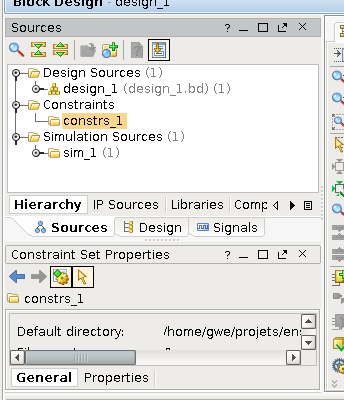
\includegraphics[width=0.4\textwidth]{addSources.png}
\end{center}
\caption{Adding constraints for mapping signals to FPGA pins.}
\label{addSources}
\end{figure}

%\section{Connecting clock and reset signals}
%
%The {\tt ltc2145} and {\tt ad9767} blocks require clock and reset signal to operate
%properly:
%
%For the ADC:
%\begin{itemize}
%\item {\tt processing\_rst\_i} must be connected to the {\tt
%adc\_rst\_o} signal of the {\tt redpitaya\_adc\_clk};
%\item {\tt resetn} must be connected to the {\tt peripheral\_aresetn} 
%signal of the {\tt Processor system Reset};
%\item {\tt adc\_clk\_i} must be connected to the {\tt adc\_clk\_o} signal of
%{\tt redpitaya\_adc\_clk}.
%\end{itemize}
%
%For the DAC:
%\begin{itemize}
%\item {\tt dac\_clk\_i} is connected to {\tt dac\_clk\_o} of {\tt
%redpitaya\_adc\_clk};
%\item {\tt dac\_2clk\_i} is connected to {\tt dac\_2clk\_o} of {\tt
%redpitaya\_adc\_clk};
%\item {\tt dac\_2ph\_i} is connected to {\tt dac\_2ph\_o} of {\tt
%redpitaya\_adc\_clk};
%\item {\tt dac\_locked\_i} is connected to {\tt dac\_locked\_o} of {\tt
%redpitaya\_adc\_clk}.
%\end{itemize}
%
%For the clock signal generator:
%\begin{itemize}
%\item {\tt adc\_rst\_i} de {\tt redpitaya\_adc\_dac\_clk} is connected to {\tt 
%peripheral\_reset} of {\tt proc\_sys\_reset}
%\end{itemize}
%
%Connect the output of the ADC to the input of the DAC:
%\begin{itemize}
%\item {\tt dataA\_out} of the ltc2145 is connected to {\tt dataA\_in} of {\tt ad9767}
%\item {\tt dataB\_out} of the ltc2145 is connected to {\tt dataB\_in} of {\tt ad9767}
%\end{itemize}

%\section{Other connections}
%
%Designs communicating between PL and PS through the AXI bus allow for automated
%routing of some of the signals. Lacking such functionalities here, we must connect
%manually:
%\begin{itemize}
%\item the {\tt FCLK\_CLK0} signal of {\tt processing\_system7\_0} is connected to
%	\begin{itemize}
%	\item {\tt M\_AXI\_GP0\_ACLK} signal of the same block,
%	\item {\tt slowest\_sync\_clk} signal of the {\tt rst\_processing\_system7\_0\_125M} block.
%	\end{itemize}
%\item the signal {\tt FCLK\_RESET0\_N} of {\tt processing\_system7\_0} is connected to the
%{\tt ext\_reset\_in} signal of the {\tt rst\_processing\_system7\_0\_125M} block.
%\end{itemize}

\section{Bitstream generation}

The project is now completed, but prior to generating the bitstream a last step
is mandatory: creating a wrapper whose function is to assemble the various HDL source
codes. This file also provides the {\tt top} file of the design.

Such a result is achieved by right-clicking in the {\tt Sources} tab the name
of the block design (Fig. \ref{createHDLWrapper}) and selecting {\tt Create HDL Wrapper}.
Having completed this step, we click on {\tt Generate Bitstream} in the lower left part of the {\tt Vivado}
graphical interface.

\begin{figure}[h!tb]
\begin{center}
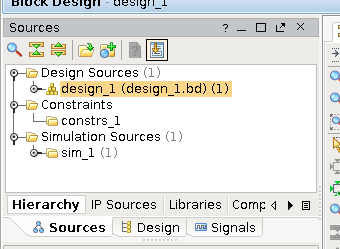
\includegraphics[width=0.5\textwidth]{createHDLWrapper.png}
\end{center}
\caption{Creating the wrapper ({\tt top} of the design) needed to generate the
bitstream}.
\label{createHDLWrapper}
\end{figure}

\section{Signed bitstream and FPGA configuration}

The previous steps have ended with the generation of a {\tt .bit} located in
the \\{\tt project\_name/project\_name.runs/impl\_1} directory and called 
{\tt project\_name\_wrapper.bit}

\subsection{Creating the encrypted bitstream}

The default file format of the bitstream generated by Vivado is a {\tt .bit} file.
The driver allowing to configure the PL from GNU/Linux requires a specific format
including a dedicated header. Converting from one format to another is achieved by
using the {\tt bootgen} tool provided by the Vivado SDK.

This tool expects a configuration file with a {\tt .bif} extension and filled with
\begin{lstlisting}
all:
{
  bitstream_name.bit
}
\end{lstlisting}

so that the following command is executed
\begin{lstlisting}[language=bash]
bootgen -image bif_file.bif -arch zynq -process_bitstream bin
\end{lstlisting}

Following this command, a file named {\tt bitstream\_name.bit.bin} is generated in
the current working directory.

\subsection{Configuring the PL by using {\tt fpga\_manager}}

GNU/Linux provides a homogeneous framework for configuring the FPGA of SoC chips: {\tt fpga\_manager}.
This framework expects the {\tt .bit.bin} file to be located in the {\tt /lib/firmware} of the
target platform.

Once the file is in the right location, the driver must be informed that the
FPGA must be configured and which bitstream to use:
\begin{lstlisting}[language=bash]
echo "bitstream_name.bit.bin" > /sys/class/fpga_manager/fpga0/firmware
\end{lstlisting}
which results in
\begin{lstlisting}[language=bash]
fpga_manager fpga0: writing bitstream_name.bit.bin to Xilinx Zynq FPGA Manager
\end{lstlisting}
being displayed in the console or in {\tt /var/log/syslog} and the LED (blue on the
Redpitaya platform) connected to {\tt Prog done} will be lit.

\subsection{Using the {\tt devicetree} overlay for PL configuration}

The devicetree overlay provides an alternative solution for configuring the FPGA in which
all necessary resources -- driver name, address space and bitstream name -- are referenced
in a single file and communicated to the kernel module.
For the purpose of this design, this solution is oversized but offer a
coherent approach with next tutorials, where Axi based IPs are used.

Similar to the previous method, the bitstream must be located in {\tt /lib/firmware}.

Without getting in the details of the devicetree overlay format, the following code aims at
modify {\tt fpga\_full} node, defined at board's default devicetree, to provide,
through attribute {\tt firmware-name}, the bitstream name.
%
%\begin{itemize}
%\item update the {\tt fpga\_full} node ({\tt target} attribute), matching the {\tt fpga\_manager}
%location of the bitstream name {\tt firmware-name};
%\item add sub-nodes defining the drivers needed to communicate with the PL and hence insert
%them in the kernel. In this example, the needed driver is {\tt gpio\_ctl} ({\tt compatible} field), 
%whose base address (0x43C00000) and range (0x1f) are filled in the {\tt reg} attribute.
%\end{itemize}\vspace{0.3cm}
 
\begin{lstlisting}
/dts-v1/;
/plugin/;
/ {
    compatible = "xlnx,zynq-7000";
    fragment@0 {
        target = <&fpga_full>;
        #address-cells = <1>;
        #size-cells = <1>;
        __overlay__ {
            #address-cells = <1>;
            #size-cells = <1>;

            firmware-name = "bitstream_name.bit.bin";
        };
    };
};
\end{lstlisting}
%            gpio1: gpio@43C00000 {
%                compatible = "gpio_ctl";
%                reg = <0x43C00000 0x0001f>;
%                gpio-controller;
%                #gpio-cells = <1>;
%                ngpio= <8>;
%            };
%        };
%    };
%};
%\end{lstlisting}

This file is compiled by using the following command
\begin{lstlisting}
/somewhere/buildroot/output/host/bin/dtc -@ -I dts -O dtb -o ${FILENAME}.dtbo ${FILENAME}.dts
\end{lstlisting}
in which 
\begin{itemize}
\item {\tt -@} requires generating symbols that will be dynamically linked when loaded,
\item {\tt -I dts} defines the format of the input file,
\item {\tt -O dtb} defines the format of the output file,
\item {\tt -o} the name of the generated file.
\end{itemize}

Loading this file in memory is achieved in two steps:
\begin{enumerate}
\item creating a directory hosting our overlay
\begin{lstlisting}[language=bash]
mkdir /sys/kernel/config/device-tree/overlays/myname
\end{lstlisting}
will create a directory automatically filled with the files needed to
communicate with the driver
\begin{lstlisting}[language=bash]
redpitaya> ls -l /sys/kernel/config/device-tree/overlays/myname/
total 0
-rw-r--r--    1 root     root             0 Jan  1 00:04 dtbo
-rw-r--r--    1 root     root          4096 Jan  1 00:04 path
-r--r--r--    1 root     root          4096 Jan  1 00:04 status
\end{lstlisting}
\item
loading the overlay in the {devicetree}~:
\begin{lstlisting}[language=bash]
cat gpio_red.dtbo > /sys/kernel/config/device-tree/overlays/myname/dtbo
\end{lstlisting}
will configure the PL by transferring the bitstream, insert, if needed, the associated module driver
as defined by the ``compatible'' field which must be filled with a matching string in
the driver.
\end{enumerate}

Returning to a state where the overlay functionalities are removed is achieved by
erasing the directory:
\begin{lstlisting}[language=bash]
rmdir /sys/kernel/config/device-tree/overlays/myname
\end{lstlisting}
\end{document}
